% !Mode:: "TeX:UTF-8" 

\chapter{\hei 研究现状}

\section{\hei 线搜索}
线搜索通常分为精确线搜索和不精确线搜索。如果计算$ \alpha_{k} $,使得
\begin{equation}
	f(x_{k}+\alpha_{k} d_{k})=\min_{\alpha >0} f(x_{k}+\alpha d_{k})
\end{equation}
寻找步长条件成立的方式称作精确线搜索技术。但是在实际计算中,对于一维问题的求解较为困难,所需迭代次数过多,在实际使用中,不精确线搜索使用更为广泛。在不精确线搜索中,只要函数值$ f(x) $在新的迭代点$ x_{k}+\alpha d_{k} $有一定下降即可。

常用的不精确下降准则有以下几种。
\begin{itemize}
	\item Armijo条件
	$$ 	f(x_{k}+\alpha_{k} d_{k}) \geq 	f(x_{k})+\rho \alpha_{k} g_{k}^{T} d_{k}$$
	\item Wolfe条件
	\begin{eqnarray*}
		f(x_{k}+\alpha_{k} d_{k}) \geq 	f(x_{k})+ \sigma_{1}\alpha g_{k}^{T} d_{k}\\
		g(x_{k}+\alpha_{k}d_{k})^{T}d_{k} \leq \sigma_{2} g_{k}^{T} d_{k};
	\end{eqnarray*}
	\item 强Wolfe条件
	\begin{eqnarray*}
		f(x_{k}+\alpha_{k} d_{k}) \geq 	f(x_{k})+ \sigma_{1}\alpha g_{k}^{T} d_{k}\\
		| g(x_{k}+\alpha_{k}d_{k})^{T}d_{k}| \leq \sigma_{2} g_{k}^{T} d_{k};
	\end{eqnarray*}
	
	其中$ \rho \in (0,1),0<\sigma_{1}<\sigma_{2}<1 $.
	
\end{itemize}

针对约束优化问题,还有一种重要的思想,那就是\textbf{非单调技术}。 非单调算法是一种不要求每次迭代结果严格下降却能获得更好收敛性的算法。Chamberlain等人\cite{chamberlain1982watchdog}于1982年针对约束优化问题提出了watchdog这一非单调技术的重要雏形。Grippo等人\cite{grippo1986nonmonotone}在1986年提出了一个最初的非单调技术。自此,非单调技术开始飞速发展。

\section{\hei Barzilai-Borwein 梯度法}

Barzilai-Borwein(BB) 梯度法\cite{barzilai1988two}是由加拿大皇家科学院院士、数学会前会长Borwein与其合作者Barzilai在1988年提出的一种新型梯度算法,当问题较为病态时,梯度下降法的收敛性质往往会收到很大影响,而BB方法的计算效果比最速下降法好很多,现已成为解决大规模问题的极具竞争力的一种方法。

BB步长目前在求解无约束优化问题的其它方法中也有广泛的应用, 例如信赖域方法、共轭梯度法、变尺度BFGS方法和尺度化的共轭梯度法。 此外, Barzilai-Borwein方法也用于求解其他类型的优化问题, 如约束优化问题、多目标规划、非光滑优化问题、非线性方程组的求解与张量特征值问题。

BB方法仅适用当前迭代点与上一步迭代点的信息来确定步长,把迭代公式 $ x_{k+1}=x_{k}-\alpha_{k}g_{k} $看成是
$$ x_{k+1}=x_{k}-D_{k}g_{k}$$
其中$ D_{k}=\alpha_{k}I $.为了使矩阵$ D_{k} $具有拟牛顿性质,求解问题
$$ \min_{\alpha_{k}} \| s_{k-1}-D_{k}y_{k-1} \|_{2}$$
或者
$$ \min_{\alpha_{k}} \| D_{k}^{-1}s_{k-1}-y_{k-1} \|_{2} $$
容易验证问题的解分别为
\begin{equation}\label{BBe}
	\alpha^{\mathrm{BB} 1}_{k} \stackrel{\text { def }}{:=} \frac{\left(s^{k-1}\right)^{T} y^{k-1}}{\left(y^{k-1}\right)^{T} y^{k-1}} \quad \text { 和 } \alpha^{\mathrm{BB} 2}_{k} \stackrel{\operatorname{def}}{:=} \frac{\left(s^{k-1}\right)^{T} s^{k-1}}{\left(s^{k-1}\right)^{T} y^{k-1}},
\end{equation}
因此可以得到BB方法的两种迭代格式:
\begin{eqnarray*}
	x_{k+1} &= x_{k} -\alpha_{k}^{BB1} \nabla f(x_{k})\\
	x_{k+1} &= x_{k} -\alpha_{k}^{BB2} \nabla f(x_{k})\\
\end{eqnarray*}
我们从式\ref{BBe}注意到,计算两种 BB 步长的任何一种仅仅需要函数相邻两步的梯度信息和迭代点信息,不需要任何线搜索算法即可选取算法步长。因为这个特点,BB 方法的使用范围特别广泛。对于一般的问题,通过式\ref{BBe}计算出的步长可能过大或过小,因此我们还需将步长做上界和下界的截断,即选取$ 0<\alpha_{m}<\alpha_{M} $使得
$$  \alpha_{m} \leq \alpha_{k} \leq \alpha_{M} $$
还需注意的是,BB方法本身是非单调方法,有时也配合非单调收敛准则使用以获得更好的实际效果,我们可以通过图\ref{bfgs}了解到BB方法相对于BFGS法的优异效果。
\begin{figure}
	\centering
	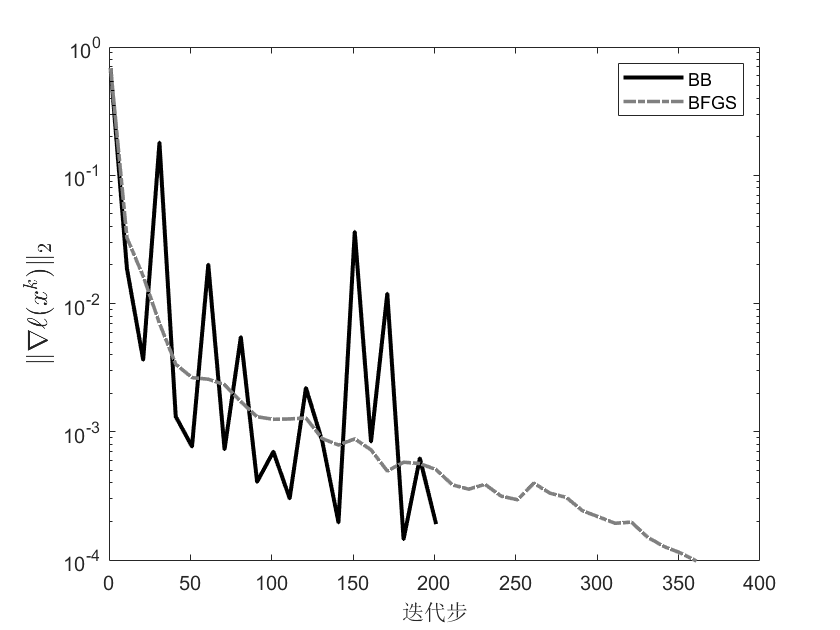
\includegraphics[scale=0.4]{BB+bfgs.png}
	\caption{BB方法与 BFGS法相对比}
	\label{bfgs}
\end{figure}

下面我们给出本次实验中非单调线搜索的BB方法的伪代码: 

\begin{algorithm}[H]
	\caption{(非单调线搜索的BB方法)}
	\floatname{algorithm}{算法}
	\renewcommand{\algorithmicrequire}{\textbf{输入:}} 
	\renewcommand{\algorithmicensure}{\textbf{输出:}}	
\end{algorithm}
(其中, $ \max _{0 \leqslant j \leqslant \min (k, M)} f\left(x^{k-j}\right) $使用回溯法寻找局部最大值)


\section{\hei 自适应步长的梯度下降方法}

BB方法在数值实验中取得了较梯度下降方法优异得多的表现。对于严格凸二次极小化问题
$$  \min_{x \in \mathbb{R}} \frac{1}{2} x^{T}Ax-b^{T}x$$
其中$ A \in \mathbb{R}^{n \times n} $是对称正定矩阵,$b \in \mathbb{R} $。Barzilai和Borwein\cite{barzilai1988two}证明了$ n=2 $时方法的R-超线性收敛性。对于$ n \leq 3 $ 的情形,Raydan\cite{raydan1993barzilai}得到了全局收敛性的结果,Dai和Liao\cite{dai2002r}进一步证明了方法是R-线性收敛的。Dai等人在\cite{dai2013new,dai2005asymptotic}讨论了BB型方法的渐进收敛性。借助于非单调线搜索\cite{grippo1991class},Raydan\cite{raydan1997barzilai}把BB方法应用到了求解一般非二次函数的极小化问题中,大量实验表明此时的BB方法可以和PRP+\cite{gilbert1992global}方法相媲美。

在以上这些方法中,我们更关注于自适应BB方法(Adaptive Barzilai–Borwein,ABB)\cite{zhou2006gradient}。

\begin{equation}\label{ABB}
	\alpha_{k}^{\text{ABB}}=\left\{
	\begin{array}{rcl}
		\alpha_{k}^{\text{BB2}},& \text{if} \quad  \dfrac{\alpha_{k}^{\text{BB2}}}{\alpha_{k}^{\text{BB1}}}<\tau \\
		\alpha_{k}^{\text{BB1}},& \text{otherwise}
	\end{array}\right.
\end{equation}



ABB方法使用一种类似信赖域的策略,从原始BB方法的两种替代公式中选择其步长,且其作为非单调算法,对于一般函数无需行行搜索,在计算无约束优化问题时可以节省大量的计算工作。在系数矩阵条件较为恶劣,并对于高精度有要求的时候,ABB方法是一个很好的备选。

为了保证全局的收敛性,我们将在下部分将ABB方法与Zhang和Hager提出的一种新型非单调线搜索技术\cite{zhang2004nonmonotone}相结合。

\section{\hei 一种新型非单调线搜索技术}

Zhang和Hager提出了一种新型非单调线搜索技术\cite{zhang2004nonmonotone},在这项技术中要求连续函数值的平均值减小,而在Grippo等人的工作\cite{grippo1986nonmonotone}中则要求最近点的函数最大值减少,即从要求
$$  f(x_{k}+\alpha_{k}d_{k}) \leq \max_{0 \leqslant j \leqslant \min (k, M)}f(x_{k-j})+\delta \alpha_{k} \nabla f(x_{k}) d_{k}$$
转变为要求
$$ f(x_{k}+\alpha_{k}d_{k}) \leq C_{k}+ \delta \alpha_{k} \nabla f(x_{k})d_{k} $$
其中,$ C_{k} $满足一定的迭代条件。
这种非单调线搜索技术具有非凸、光滑函数的全局收敛性,以及强凸函数的R-线性收敛性。相比L-BFGS方法,该技术使用更少的函数值和梯度值计算,因此性能更加优越。

下面我们给出这种新型非单调线搜索技术(Nonmonotone Line Search Algorithm,NLSA):
\begin{itemize}
	\item \textbf{初始化}:选定初始点$ x_{0} $,和参数$ 0 \leq \alpha_{min} \leq \alpha_{max} \leq 1 , 0<  \delta < \sigma <1 < \rho , \mu >0$,设定$ C_{0} = f(x_{0}),Q_{0}=1,k=0 $.
	\item \textbf{收敛性测试}:若$ \| \nabla f(x_{k}) \| $充分小,则停止迭代.
	\item \textbf{升级版线搜索}:令$ x_{k+1}=x_{k}+\alpha_{k}d_{k} $,其中$ \alpha_{k} $需满足Wolfe条件
	\begin{eqnarray*}
		f(x_{k}+\alpha_{k}d_{k}) &\leq C_{k}+ \delta \alpha_{k} \nabla f(x_{k})d_{k},\\
		\nabla f(x_{k}+\alpha_{k}d_{k})d_{k} &\geq \sigma \nabla f(x_{k})d_{k}
	\end{eqnarray*}
	或满足Armijo条件:$ \alpha_{k} = \bar{\alpha_{k}}\rho^{h_{k}} $,其中$ \bar{\alpha_{k}} >0 $是试验步,$ h_{k} $是满足$f(x_{k}+\alpha_{k}d_{k}) \leq C_{k}+ \delta \alpha_{k} \nabla f(x_{k})d_{k} $的最大整数,并且$ \alpha_{k} \leq \mu $
	\item \textbf{升级版成本}:在$ \alpha_{k} \in \left[ \alpha_{\min} ,\alpha_{\max} \right] $,并设定
	$$ Q_{k+1}=\alpha_{k}Q_{k}+1 , \qquad C_{k+1}=(\alpha_{k} Q_{k}C_{k}+f(x_{k+1}))/Q_{k+1},\qquad k:=k+1.$$
	并且重新返回进行收敛性测试。
\end{itemize}
%我们可以得知,$ C_{k+1} $是一个$ C_{k} $和$ f(x_{k+1}) $的凸组合。自$ C_{0}=f(x_{0}) $起,$ C_{k} $就是一个$ f(x_{0}),f(x_{1}), \cdots , f(x_{k}) $的凸组合。$ \alpha_{k} $的选择控制了非单调性的程度。如果每步迭代$ \alpha_{k}=0 $,线搜索就遵循通用的单调Wolfe和Armijo准则。如果每步迭代$ \alpha_{k}=1 $,则$ C_{k}=A_{k} $


\section{\hei 最终改进形式}
我们给出基于非单调线搜索的BB步长改进的最终版本伪代码:

\begin{algorithm}[H]
	\SetAlgoLined
	\KwData{计算节点client}
	\KwResult{计算文件\texttt{test.py}}
	\Begin{
		data = client.recv(1024)\\
		\eIf{data == b'exist'}{
			\eIf{os.path.exists("test.py")}{
				client.send("Y".encode('utf-8'))\\
			}{
				client.send("N".encode('utf-8'))\\
				\While{True}{
					with open("test.py", "ab") as f\\
					data = client.recv(1024)\\
					\eIf{data == b'quit'}{
						client.send("received".encode('utf-8'))\\
						break
					}{}
					f.write(data)
				}
				print("节点\%d:计算文件已经接收!存储为test.py" \% (cnt)) break
			}
		}{}
	}
	\caption{FileSplitSend()\label{chap:chap02:alg:SPLITFILE:expire}}
\end{algorithm}
并在测试函数Rosenbrock函数  $f(x)=100(x_{2}-x_{1}^{2})^{2}+(1-x_{1})^{2}  $上验证了数值效果,如图\ref{testbb}所展示。
\begin{figure}
	\centering
	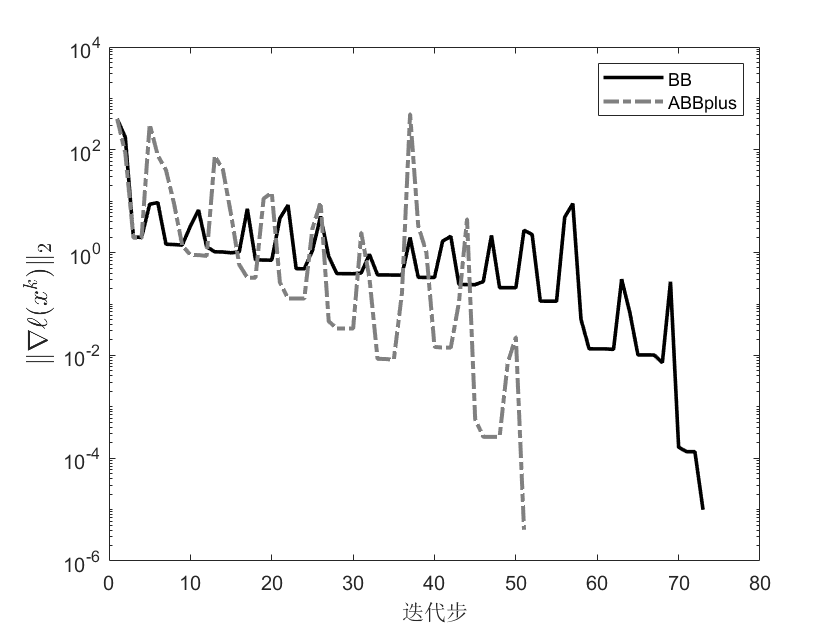
\includegraphics[scale=0.4]{test_BB+ABB_plus.png}
	\caption{由二次函数生成的$ \{ \|  g_{k} \| \} $序列}
	\label{testbb}
\end{figure}


\chapter{\hei 数值实验}

本节,我们通过数值试验来阐述以上几项改进形式在实际问题当中的数值表现。所有的代码用MATLAB R2021编写,在具有2.50GHzCPU处理器,8.00G内存,Windows 10操作系统的个人电脑上运行。


终止准则为
$$ \| \nabla f(x_{k}) \| \leq \epsilon $$

所有算法均通过以下三个数据集‘a9a.test’,‘CINA.test’,‘ijcnn1.test’进行数值实验,并据此进行算法效果对比,并通过表\ref{dataset}进行维度展示,其中我们选取a9a数据集作为实验的主数据集。


图\ref{BBq}展示了由BB方法($\mu=1 e-2 / m$)产生的梯度序列$ \{ \|  g_{k} \| \} $(取$ \log_{10} $对数之后)随迭代步数变化的情况。图形阐述了BB型方法的非单调性, 也在某种意义上说明了方法的R-线性收敛性结果.
\begin{figure}
	\centering
	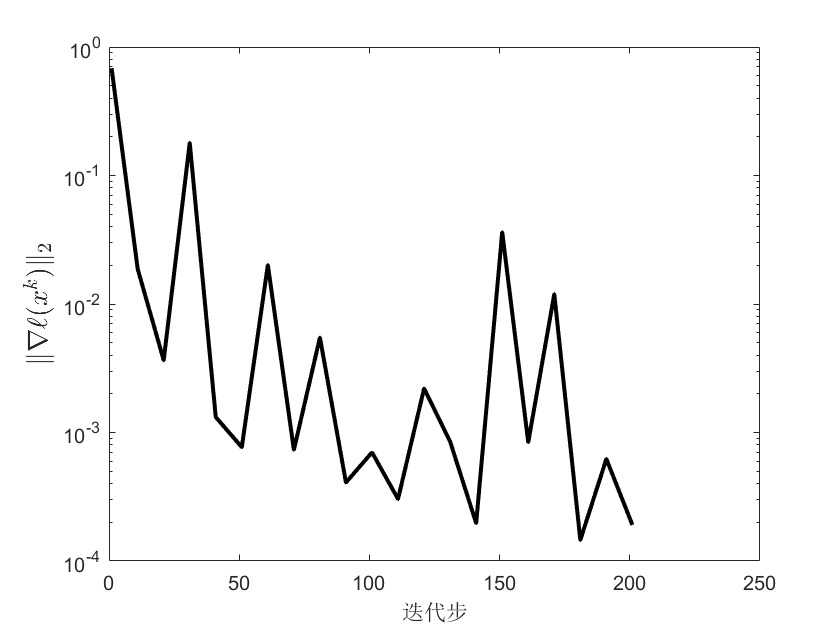
\includegraphics[scale=0.4]{BB.png}
	\caption{BB方法($\mu=1 e-2 / m$)产生的梯度序列$ \{ \|  g_{k} \| \} $}
	\label{BBq}
\end{figure}

下面我们将进一步对BB方法以及其几个改进方法进行对比,
并通过图\ref{BBcontrast}展示了各项改进相对于改进前的效果对比。

\begin{figure}[htbp]
	\centering
	\subfigure[BB与BBplus]{
		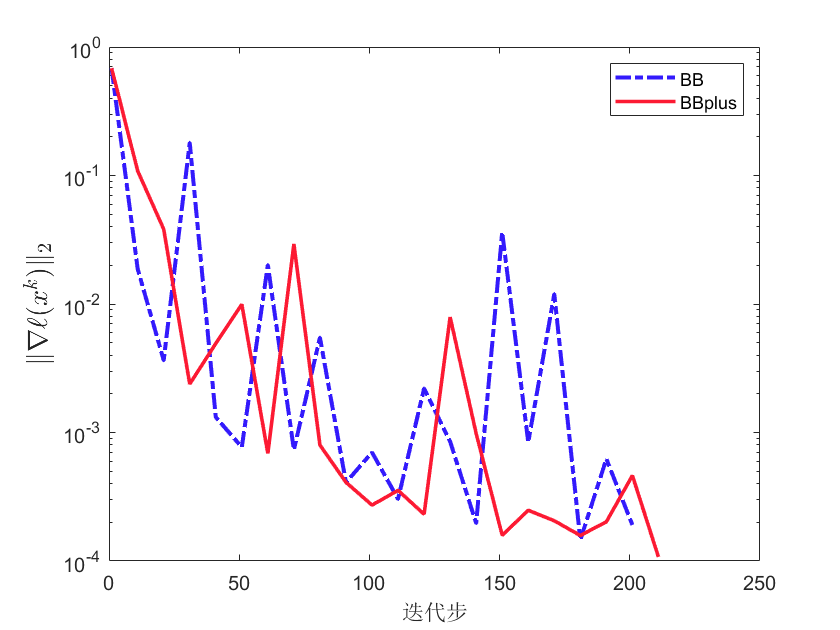
\includegraphics[width=7cm]{BB+BB_plus.png}
		\label{BBcontrast1}
		%\caption{BB与BBplus}
	}
	\quad
	\subfigure[BB与ABB]{
		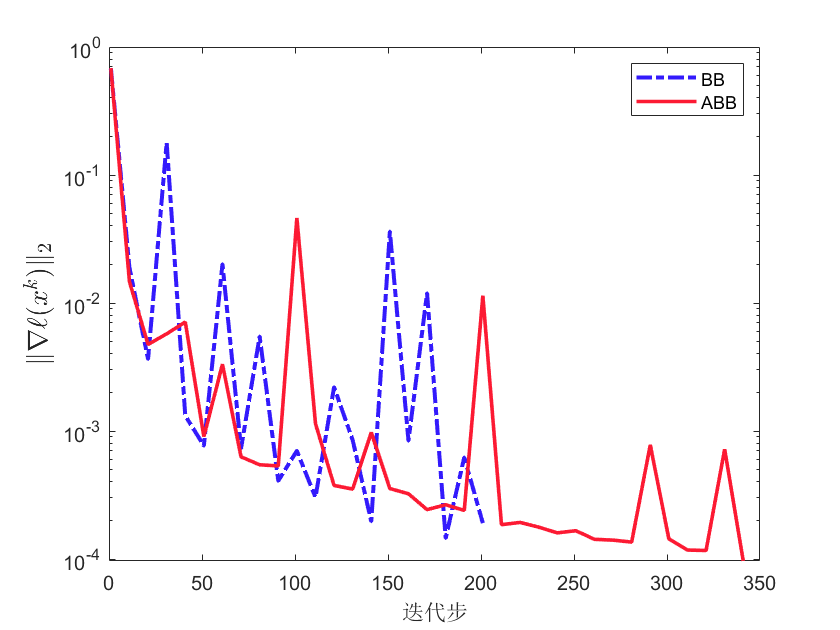
\includegraphics[width=7cm]{BB+ABB.png}
		\label{BBcontrast2}
	}
	\quad
	\subfigure[ABB与ABBplus]{
		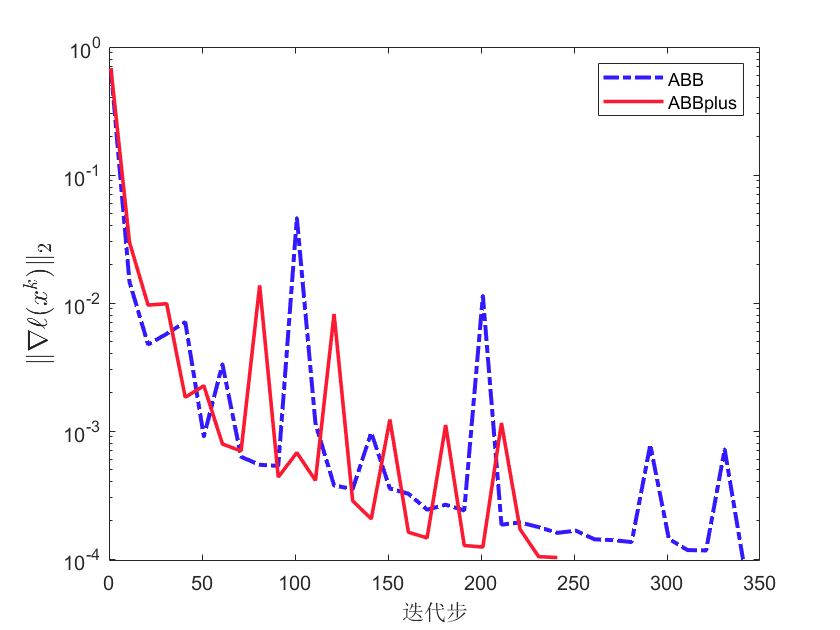
\includegraphics[width=7cm]{ABB+ABB_plus.png}
		\label{BBcontrast3}
	}
	\quad
	\subfigure[BB与ABBplus]{
		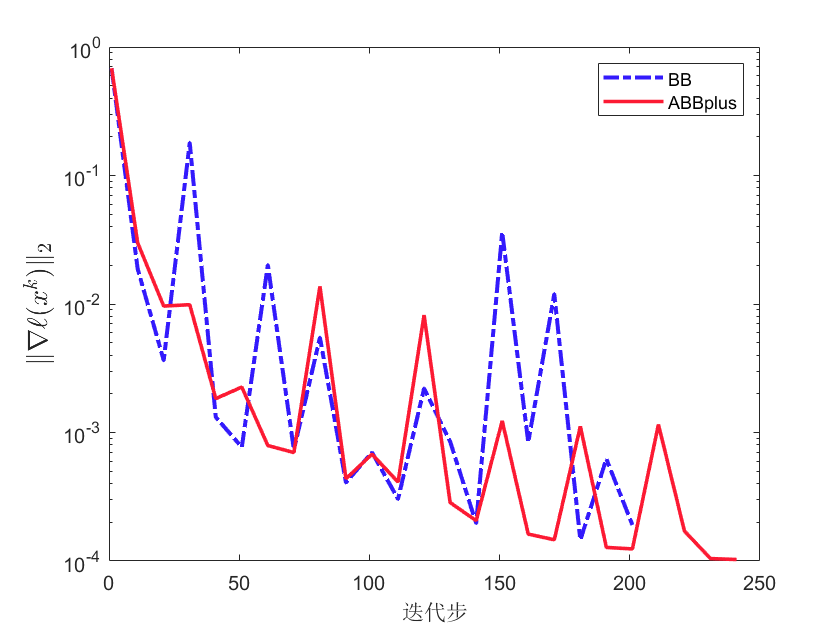
\includegraphics[width=7cm]{BB+ABB_plus.png}
		\label{BBcontrast4}
	}
	\caption{改进的BB方法与原方法$ \{ \|  g_{k} \| \} $序列对比图}
	\label{BBcontrast}	
\end{figure}

\begin{table}[thp]
	\centering
	\begin{tabular}{cccc}
		\toprule
		\hline
		& 迭代次数(次) & CPU运行时间(s) & 最终 $ \|  g_{k} \|  $ \\
		\cmidrule(lr){2-4}
		BFGS & 360 & 8.9688 & 9.8513e-05 \\
		
		BB & 207 &  7.6094 & 9.8505e-05 \\
		
		BBplus & 219 &  4.7656 & 9.7806e-05 \\
		
		ABB & 340 &  9.8594 &  9.6564e-05\\
		
		\textbf{ABBplus} & 250 & 5.1094 &  9.8973e-05\\
		\hline
	\end{tabular}
	\caption{算法对比}
	\label{al}
\end{table}

\begin{itemize}
	\item 各项改进方法均能较好的求解出实际问题且效果良好。
	\item \textbf{相对于BB方法},各项改进虽均在迭代步数上有所增加,但是却在步长选择、计算开销、全局收敛性上有了较大的提升,我们在图\ref{testbb}上也可了解到其改进效果。
	\item 各方法在三个数据集上均表现良好,如图\ref{datesetcontrast}所示。
	
	\begin{table}\centering
		\begin{tabular}{cccc}
			\toprule
			\hline
			& a9a & CINA & ijcnn1 \\
			\cmidrule(lr){2-4}
			A & 16281 $\times$ 122 & 3206$\times$132 & 91701$\times$22 \\
			
			b & 16281$\times$1 & 3206$\times$1 & 91701$\times$1 \\
			\hline
		\end{tabular}
		\caption{数据集维度展示}
		\label{dataset}
	\end{table}

\begin{figure}[htbp]
	\centering
	\subfigure[BB]{
		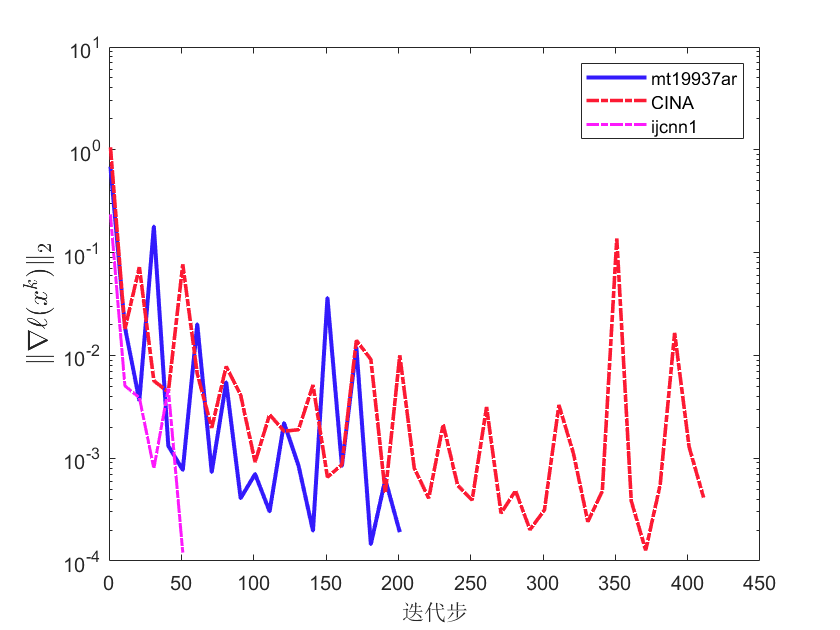
\includegraphics[width=7cm]{BB_dataset.png}
		\label{datesetcontrast1}
		%\caption{BB与BBplus}
	}
	\quad
	\subfigure[BBplus]{
		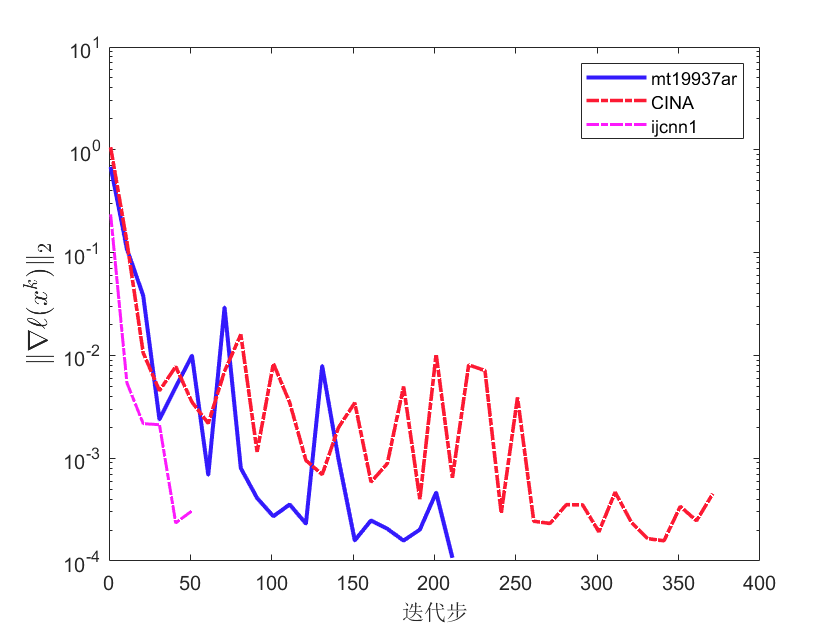
\includegraphics[width=7cm]{BBplus_dataset.png}
		\label{datesetcontrast2}
	}
	\quad
	\subfigure[ABB]{
		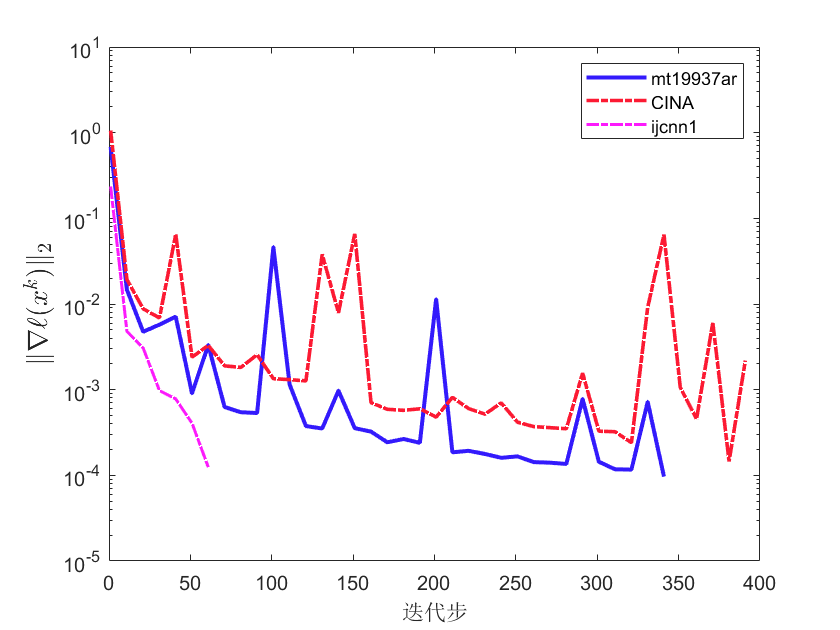
\includegraphics[width=7cm]{ABB_dataset.png}
		\label{datesetcontrast3}
	}
	\quad
	\subfigure[ABBplus]{
		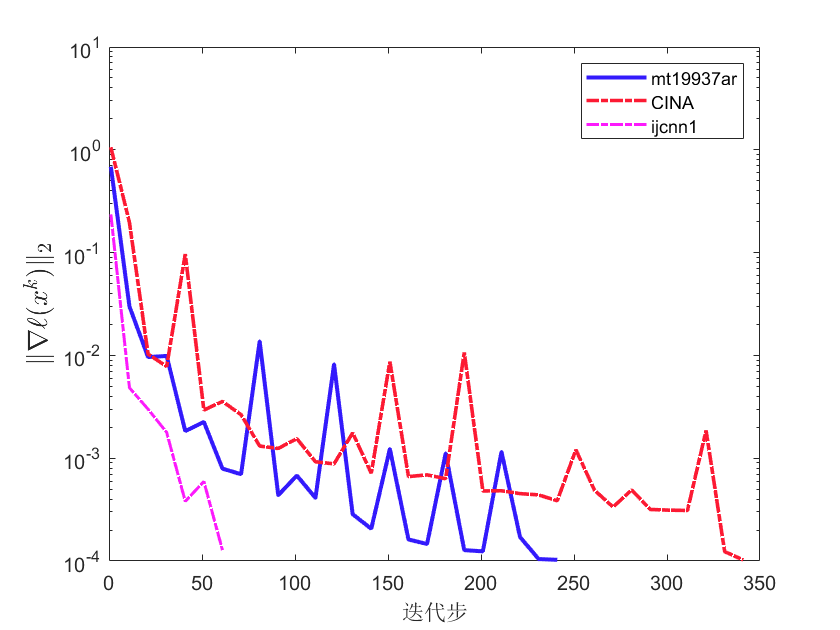
\includegraphics[width=7cm]{ABBplus_dataset.png}
		\label{datesetcontrast4}
	}
	\caption{三个数据集验证$ \{ \|  g_{k} \| \} $序列对比图}
	\label{datesetcontrast}
\end{figure}

\item 我们还对自适应步长的BB方法(ABB)公式\ref{ABB}中的参数$ \tau \in (0,1)$产生了兴趣,并对其进行了调整测试,具体结果可由表\ref{ABBtau}可知。如无特殊说明,本次实验中ABB算法的$ \tau =0.5$。

\begin{table}[thp]
	\centering
	\begin{tabular}{cccc}
		\toprule
		\hline
		& 迭代次数(次) & CPU运行时间(s) & 最终 $ \|  g_{k} \|  $ \\
		\cmidrule(lr){2-4}
		0.1 & 328 & 14.0871 & 9.9887e-05 \\
		
		0.3 & 287 &  12.3906 & 9.9184e-05 \\
		
		0.5 & 340 &  9.8594 & 96564e-05 \\
		
		0.7 & 296 &  13.4844 &  9.7743e-05\\
		
		0.9 & 224 & 9.2813 &  9.9791e-05\\
		\hline
	\end{tabular}
	\caption{ABB中参数$ \tau $调整效果对比}
	\label{ABBtau}
\end{table}

\item 我们从表\ref{al}可知,\textbf{最终改进}结果的算法ABBplus既保证了在不大规模增加迭代次数的情况下提升了求解精度,又极大的节省了计算开销,计算时间相对于原始BB方法而言减少了48.9\% ,相对于ABB方法而言更是减少了93.0\%。



\item 从图\ref{time}可以观察到,就\textbf{任务完成度}而言,在CPU运行时间到达第5秒时,算法BBplus和ABBplus已经分别完成了计算任务的100\% 和 97.9\%,而BB方法和BFGS方法则仅仅完成了整体计算任务的65.7\%和55.7\%。


\item 同时为了算法调优,我们对\textbf{正则化系数$ m $}进行了调整,见下表\ref{m}。我们可以观察到,随着正则化系数的增加,迭代次数大幅度下降,但是精度也随之下降。迭代次数下降的原因我们猜测由于测试函数本身属性的影响,具体原因还有待具体研究。\\
从上述调整的参数来看,正则化系数在被选择为$ 1/m $附近时,迭代次数较少、CPU运行时间较低,同时维持了一个较好的精度。
\end{itemize}

\begin{figure}
	\centering
	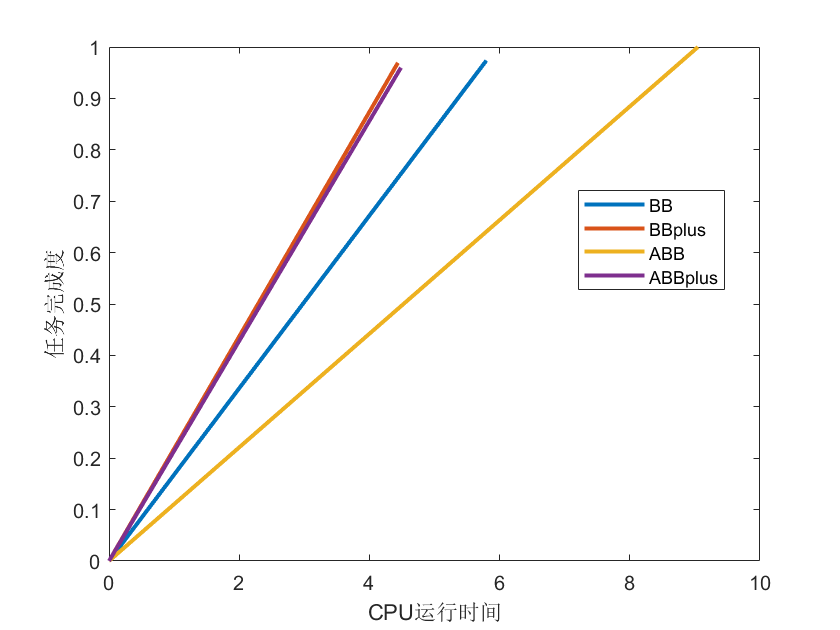
\includegraphics[scale=0.4]{time.png}
	\caption{BB方法及其改进基于CPU时间的对比}
	\label{time}
\end{figure}
%%%%%%%%%%%%%%%%%%%%%%%%%%%%%%%%%%%%%%%%%%%%%%%%%%%%%%%%%%%%


\chapter{\hei 小结}

本次报告主要研究BB型步长及其改进形式在优化算法中的应用。
首先,我们实现了基于Grippo等人提出的非单调技术\cite{grippo1991class}的BB型步长\cite{barzilai1988two}和自适应步长BB方法(ABB)\cite{zhou2006gradient}。
其次,我们将由Zhang和Hager提出的一种新型非单调线搜索技术\cite{zhang2004nonmonotone}分别应用到BB方法和ABB方法上,在极大减少ABB方法迭代次数的同时,吸收了BB方法的非单调及高精度等优点,在多项数值实验上取得了优异的效果。
最后,我们还关注了不同数量级正则化系数对于逻辑回归函数的影响,并针对数值结果选取了表现相对优异的系数。